% ===================================================================
% FIGURE: HE Chain Depth Accuracy (from EH3 depth study)
% Shows max error remains stable across depths 1-5
% Requires: \usepackage{pgfplots} in preamble
% ===================================================================

\begin{figure}[t]
\centering
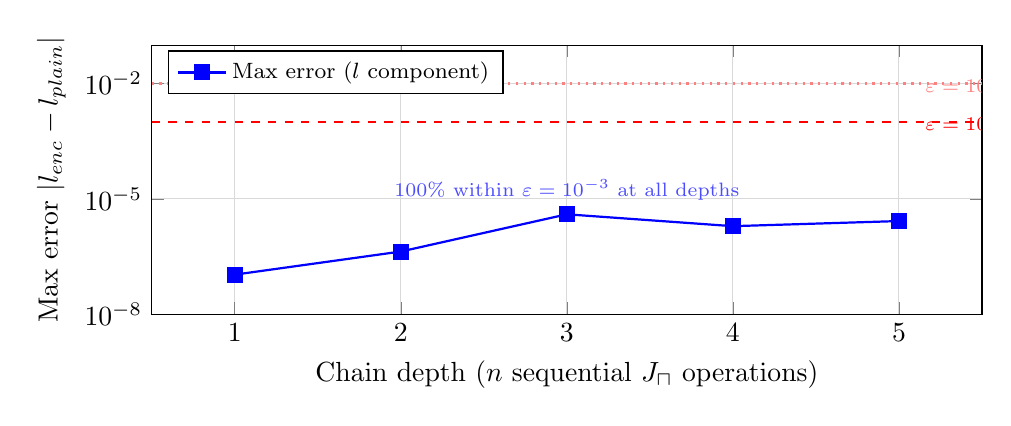
\begin{tikzpicture}
\begin{axis}[
    width=\columnwidth,
    height=5cm,
    xlabel={Chain depth ($n$ sequential $J_\sqcap$ operations)},
    ylabel={Max error $|l_{\text{enc}} - l_{\text{plain}}|$},
    ymode=log,
    xmin=0.5, xmax=5.5,
    ymin=1e-8, ymax=1e-1,
    xtick={1,2,3,4,5},
    legend style={at={(0.02,0.98)}, anchor=north west, font=\footnotesize},
    grid=major,
    grid style={gray!30},
    every axis plot/.append style={thick},
]

% Max error per depth
\addplot[blue, mark=square*, mark size=2.5pt]
    coordinates {
        (1, 1.07e-07)
        (2, 4.27e-07)
        (3, 3.97e-06)
        (4, 1.95e-06)
        (5, 2.65e-06)
    };
\addlegendentry{Max error ($l$ component)}

% Threshold lines
\addplot[red, dashed, domain=0.5:5.5] {0.001};
\addplot[red!50, dotted, domain=0.5:5.5] {0.01};

\node[font=\scriptsize, red, anchor=west] at (axis cs:5.1, 0.001) {$\varepsilon = 10^{-3}$};
\node[font=\scriptsize, red!50, anchor=west] at (axis cs:5.1, 0.01) {$\varepsilon = 10^{-2}$};

% Annotation
\node[font=\scriptsize, anchor=south, text=blue!70] at (axis cs:3, 5e-6)
    {100\% within $\varepsilon = 10^{-3}$ at all depths};

\end{axis}
\end{tikzpicture}
\caption{CKKS encrypted $J_\sqcap$ accuracy across chain depths. Max error over 100 trials per depth remains below $\varepsilon = 10^{-3}$ through depth 5, demonstrating that noise accumulation is well-managed by automatic parameter scaling. Overhead: $15{,}186\times$ vs.\ plaintext (27\,ms vs.\ 0.002\,ms).}
\label{fig:he_depth}
\end{figure}
